%!TEX root = /Users/kevin/SkyDrive/KTH Work/Period 4 2014/GNSS/Labs/L4 - Kalman filtering/main.tex


\section{Results} % (fold)
\label{sec:results}
A comparison of the filtered and smoothed coordinates with the true measurements are shown in Figures~\ref{fig:Figures_xDataPlots} and \ref{fig:Figures_vDataPlots}. Table~\ref{tab:tableFiltered.tex} and~\ref{tab:tableSmoothed.tex} are the coordinates after filtering and smoothing.  Figures~\ref{fig:Figures_diffPlots} and \ref{fig:Figures_diffPlotsVelocity} show the difference between the true measurements and the filtered and smoothed results.
\begin{figure}[htbp]
	\centering
		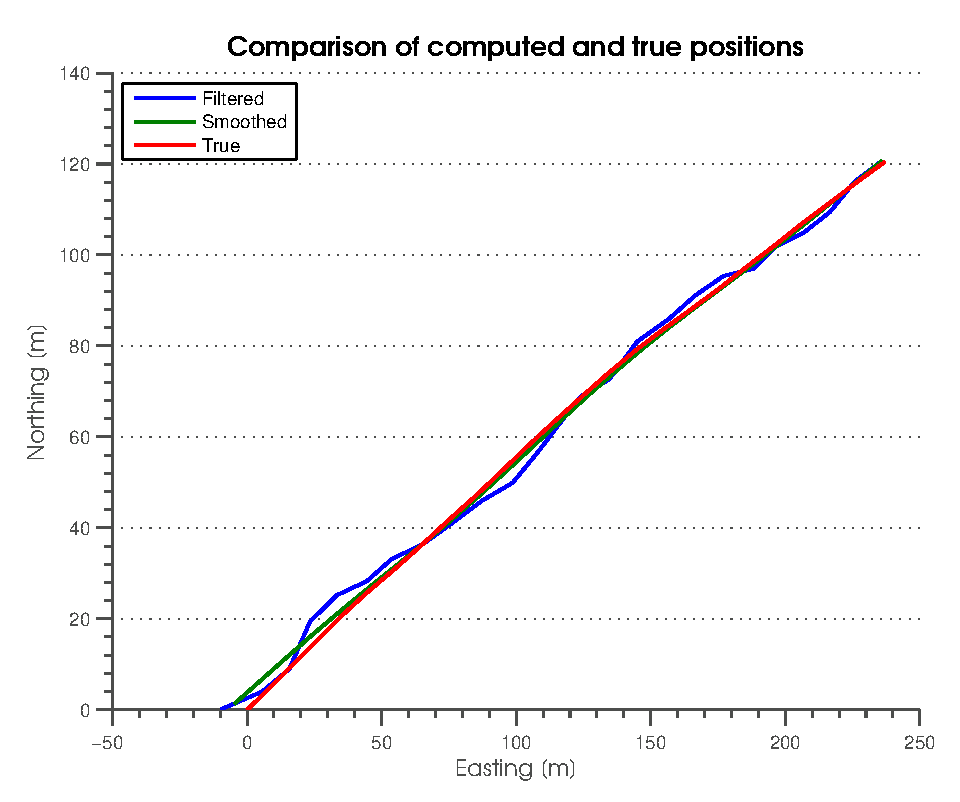
\includegraphics[width=\MyWidth]{Figures/xDataPlots.eps}
	\caption{Comparison of filtered, smoothed, original, and true coordinates.}
	\label{fig:Figures_xDataPlots}
\end{figure} % (fig:Figures_xDataPlots)
\begin{figure}[htbp]
	\centering
		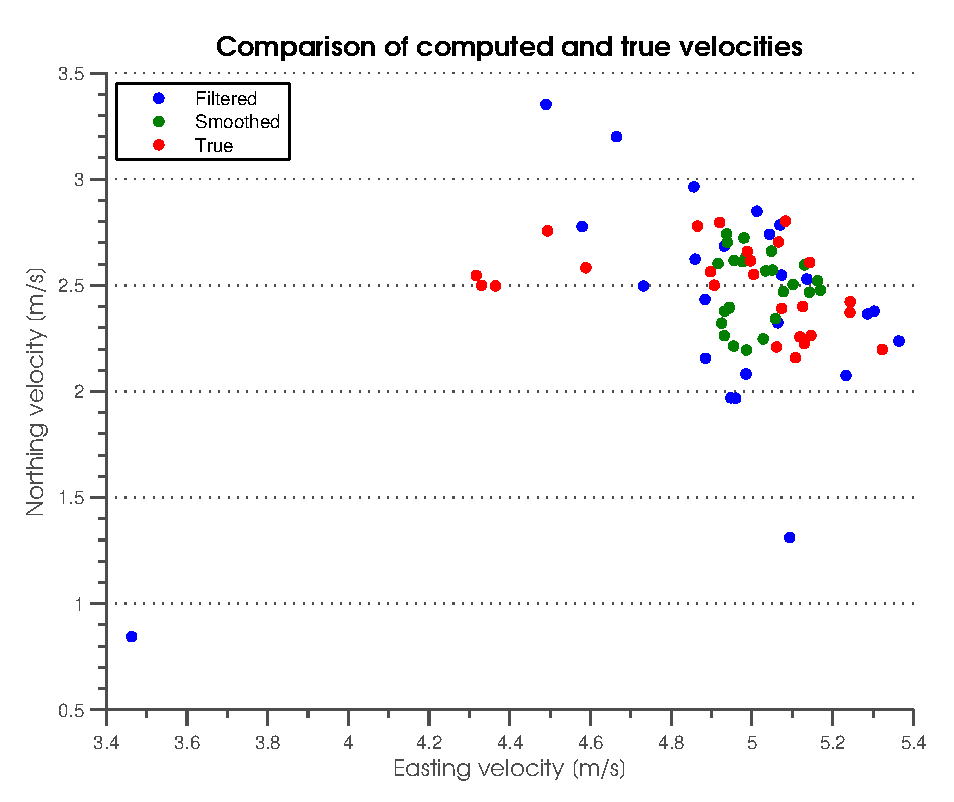
\includegraphics[width=\MyWidth]{Figures/vDataPlots.eps}
	\caption{Comparison of filtered, smoothed, and true velocities.}
	\label{fig:Figures_vDataPlots}
\end{figure} % (fig:Figures_vDataPlots)
\begin{table}[h] 
   \begin{center} 
      \begin{tabular}{lllllllll}\toprule 
\multicolumn{5}{c}{Filtered Estimations and standard deviations}\\ 
\midrule 
t&  $x_e \pm \sigma_e$& $x_n \pm \sigma_n$& $v_e \pm \sigma_{v_e}$& $v_n \pm \sigma_{v_n}$\\ \midrule 
0 & $   -9.62 \pm    10.00$ & $    0.11 \pm    10.00$ & $    3.46 \pm     3.00$ & $    0.84 \pm     3.00$  \\ 
2 & $    5.71 \pm     1.71$ & $    4.00 \pm     1.71$ & $    5.09 \pm     0.90$ & $    1.31 \pm     2.52$  \\ 
4 & $   15.74 \pm     1.33$ & $    8.98 \pm     1.64$ & $    4.95 \pm     0.51$ & $    1.97 \pm     1.05$  \\ 
6 & $   23.36 \pm     1.23$ & $   19.32 \pm     1.53$ & $    4.49 \pm     0.37$ & $    3.35 \pm     0.58$  \\ 
8 & $   33.40 \pm     1.19$ & $   25.17 \pm     1.42$ & $    4.66 \pm     0.30$ & $    3.20 \pm     0.40$  \\ 
10 & $   44.56 \pm     1.17$ & $   28.26 \pm     1.31$ & $    4.93 \pm     0.27$ & $    2.68 \pm     0.31$  \\ 
12 & $   53.82 \pm     1.15$ & $   33.15 \pm     1.24$ & $    4.86 \pm     0.25$ & $    2.62 \pm     0.27$  \\ 
14 & $   65.20 \pm     1.13$ & $   36.34 \pm     1.19$ & $    5.06 \pm     0.24$ & $    2.32 \pm     0.25$  \\ 
16 & $   76.79 \pm     1.11$ & $   41.27 \pm     1.16$ & $    5.30 \pm     0.23$ & $    2.38 \pm     0.24$  \\ 
18 & $   87.52 \pm     1.09$ & $   46.04 \pm     1.14$ & $    5.29 \pm     0.23$ & $    2.37 \pm     0.24$  \\ 
20 & $   98.70 \pm     1.09$ & $   49.89 \pm     1.13$ & $    5.36 \pm     0.23$ & $    2.24 \pm     0.24$  \\ 
22 & $  107.87 \pm     1.08$ & $   56.46 \pm     1.13$ & $    5.14 \pm     0.23$ & $    2.53 \pm     0.24$  \\ 
24 & $  117.40 \pm     1.08$ & $   63.85 \pm     1.13$ & $    5.01 \pm     0.23$ & $    2.85 \pm     0.24$  \\ 
26 & $  124.41 \pm     1.08$ & $   69.08 \pm     1.13$ & $    4.58 \pm     0.23$ & $    2.78 \pm     0.24$  \\ 
28 & $  134.62 \pm     1.08$ & $   72.63 \pm     1.13$ & $    4.73 \pm     0.23$ & $    2.50 \pm     0.24$  \\ 
30 & $  145.07 \pm     1.08$ & $   81.00 \pm     1.13$ & $    4.86 \pm     0.23$ & $    2.96 \pm     0.24$  \\ 
32 & $  156.58 \pm     1.08$ & $   85.84 \pm     1.13$ & $    5.07 \pm     0.23$ & $    2.78 \pm     0.24$  \\ 
34 & $  166.60 \pm     1.08$ & $   91.13 \pm     1.12$ & $    5.04 \pm     0.23$ & $    2.74 \pm     0.24$  \\ 
36 & $  177.15 \pm     1.08$ & $   95.37 \pm     1.12$ & $    5.07 \pm     0.23$ & $    2.55 \pm     0.24$  \\ 
38 & $  188.30 \pm     1.08$ & $   97.05 \pm     1.12$ & $    5.23 \pm     0.23$ & $    2.07 \pm     0.24$  \\ 
40 & $  196.25 \pm     1.08$ & $  101.75 \pm     1.13$ & $    4.89 \pm     0.23$ & $    2.16 \pm     0.24$  \\ 
42 & $  206.72 \pm     1.08$ & $  104.80 \pm     1.13$ & $    4.96 \pm     0.23$ & $    1.97 \pm     0.24$  \\ 
44 & $  216.74 \pm     1.08$ & $  109.52 \pm     1.13$ & $    4.99 \pm     0.23$ & $    2.08 \pm     0.24$  \\ 
46 & $  225.83 \pm     1.08$ & $  116.11 \pm     1.13$ & $    4.88 \pm     0.23$ & $    2.43 \pm     0.24$  \\ 
48 & $  236.10 \pm     1.08$ & $  120.72 \pm     1.13$ & $    4.94 \pm     0.23$ & $    2.39 \pm     0.24$  \\ \bottomrule 
      \end{tabular} 
   \end{center}
\caption{The easting and northing coordinates and velocities are given with their standard deviations.} 
\label{tab:tableFiltered.tex} 
\end{table} 

\begin{table}[h] 
   \begin{center} 
      \begin{tabular}{lllllllll}\toprule 
\multicolumn{5}{c}{Smoothed Estimations and standard deviations}\\ 
\midrule 
t&  $x_e \pm \sigma_e$& $x_n \pm \sigma_n$& $v_e \pm \sigma_{v_e}$& $v_n \pm \sigma_{v_n}$\\ \midrule 
0 & $    5.20 \pm     1.22$ & $    1.26 \pm     1.53$ & $    4.92 \pm     0.81$ & $    2.60 \pm     2.47$  \\ 
2 & $   15.13 \pm     0.42$ & $    6.48 \pm     0.37$ & $    4.96 \pm     0.37$ & $    2.62 \pm     0.97$  \\ 
4 & $   25.14 \pm     0.62$ & $   11.72 \pm     0.41$ & $    4.98 \pm     0.19$ & $    2.61 \pm     0.46$  \\ 
6 & $   35.28 \pm     0.62$ & $   16.90 \pm     0.37$ & $    5.03 \pm     0.07$ & $    2.57 \pm     0.24$  \\ 
8 & $   45.53 \pm     0.60$ & $   21.97 \pm     0.46$ & $    5.10 \pm     0.07$ & $    2.50 \pm     0.10$  \\ 
10 & $   55.84 \pm     0.59$ & $   26.94 \pm     0.53$ & $    5.14 \pm     0.10$ & $    2.47 \pm     0.08$  \\ 
12 & $   66.18 \pm     0.60$ & $   31.88 \pm     0.58$ & $    5.17 \pm     0.12$ & $    2.48 \pm     0.12$  \\ 
14 & $   76.48 \pm     0.61$ & $   36.87 \pm     0.61$ & $    5.16 \pm     0.12$ & $    2.52 \pm     0.13$  \\ 
16 & $   86.66 \pm     0.62$ & $   41.99 \pm     0.63$ & $    5.13 \pm     0.13$ & $    2.60 \pm     0.13$  \\ 
18 & $   96.69 \pm     0.63$ & $   47.24 \pm     0.65$ & $    5.05 \pm     0.13$ & $    2.66 \pm     0.13$  \\ 
20 & $  106.60 \pm     0.64$ & $   52.63 \pm     0.65$ & $    4.98 \pm     0.13$ & $    2.72 \pm     0.13$  \\ 
22 & $  116.47 \pm     0.64$ & $   58.11 \pm     0.65$ & $    4.94 \pm     0.13$ & $    2.74 \pm     0.13$  \\ 
24 & $  126.38 \pm     0.64$ & $   63.56 \pm     0.65$ & $    4.94 \pm     0.13$ & $    2.70 \pm     0.13$  \\ 
26 & $  136.43 \pm     0.65$ & $   68.90 \pm     0.65$ & $    4.98 \pm     0.13$ & $    2.64 \pm     0.13$  \\ 
28 & $  146.56 \pm     0.64$ & $   74.11 \pm     0.65$ & $    5.05 \pm     0.13$ & $    2.57 \pm     0.13$  \\ 
30 & $  156.71 \pm     0.65$ & $   79.17 \pm     0.65$ & $    5.08 \pm     0.13$ & $    2.47 \pm     0.13$  \\ 
32 & $  166.79 \pm     0.64$ & $   83.98 \pm     0.66$ & $    5.06 \pm     0.13$ & $    2.34 \pm     0.13$  \\ 
34 & $  176.81 \pm     0.65$ & $   88.56 \pm     0.66$ & $    5.03 \pm     0.13$ & $    2.25 \pm     0.13$  \\ 
36 & $  186.75 \pm     0.65$ & $   92.99 \pm     0.67$ & $    4.99 \pm     0.13$ & $    2.19 \pm     0.13$  \\ 
38 & $  196.63 \pm     0.65$ & $   97.39 \pm     0.67$ & $    4.95 \pm     0.13$ & $    2.21 \pm     0.14$  \\ 
40 & $  206.49 \pm     0.65$ & $  101.87 \pm     0.67$ & $    4.93 \pm     0.14$ & $    2.26 \pm     0.14$  \\ 
42 & $  216.34 \pm     0.67$ & $  106.45 \pm     0.68$ & $    4.93 \pm     0.15$ & $    2.32 \pm     0.15$  \\ 
44 & $  226.22 \pm     0.73$ & $  111.15 \pm     0.74$ & $    4.93 \pm     0.16$ & $    2.38 \pm     0.17$  \\ 
46 & $  236.10 \pm     0.85$ & $  115.93 \pm     0.88$ & $    4.94 \pm     0.19$ & $    2.40 \pm     0.20$  \\ \bottomrule 
      \end{tabular} 
   \end{center}
\caption{The easting and northing coordinates and velocities are given with their standard deviations.} 
\label{tab:tableSmoothed.tex} 
\end{table} 

\begin{figure}[h]
	\centering
		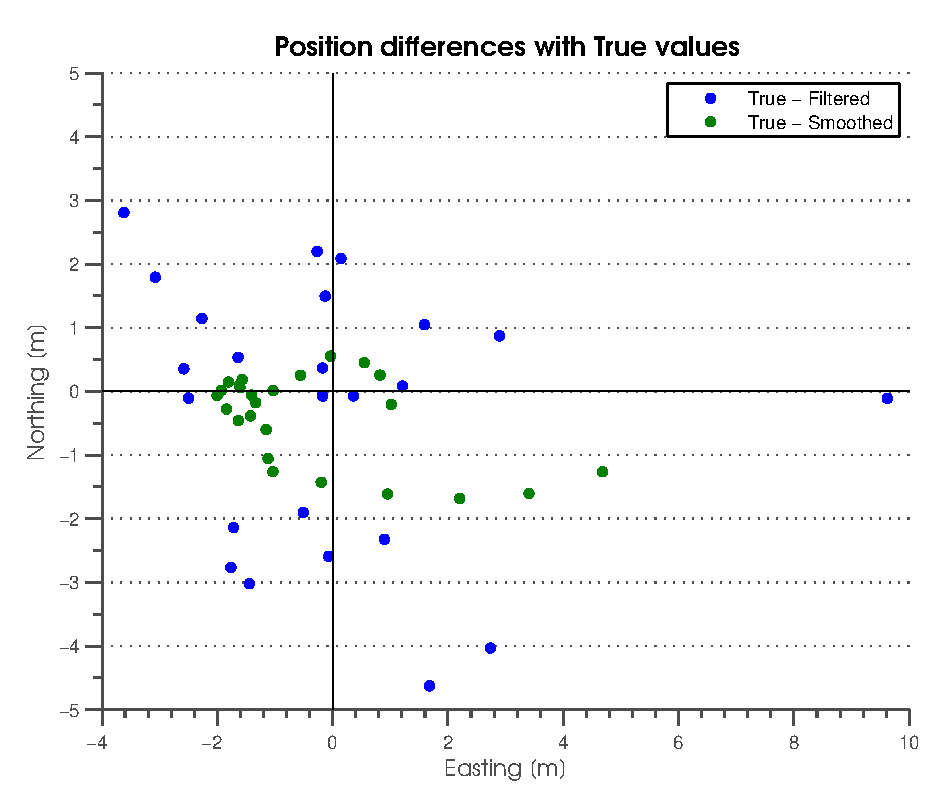
\includegraphics[width=\MyWidth]{Figures/diffPlots.eps}
	\caption{Plot of differences between true values and the filtered and smoothed coordinates.}
	\label{fig:Figures_diffPlots}
\end{figure} % (fig:Figures_diffPlots)
\begin{figure}[h]
	\centering
		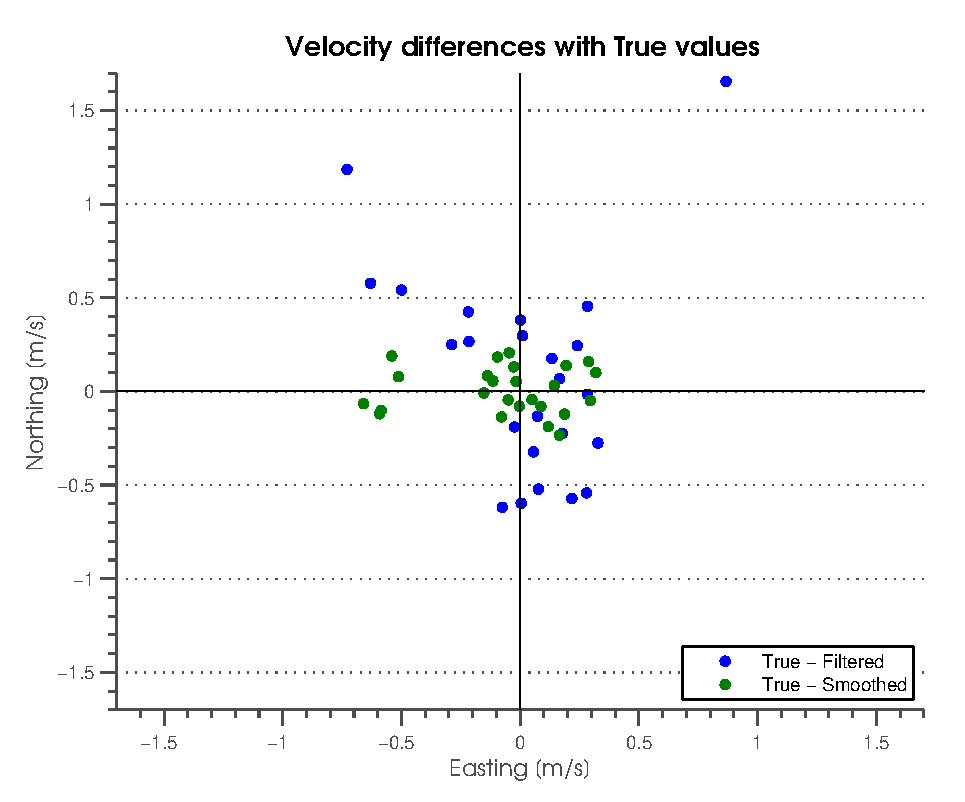
\includegraphics[width=\MyWidth]{Figures/diffPlotsVelocity.eps}
	\caption{Plot of differences between true values and the filtered and smoothed velocities.}
	\label{fig:Figures_diffPlotsVelocity}
\end{figure} % (fig:Figures_diffPlotsVelocity)
% section results (end)
